%********** Chapter 2 **********
\chapter{Background}

\section{Motivation}

3D scene reconstruction from 2D images has been an old and challenging problem. The task of computer vision and image processing is to be able to bring sight to the computer and provide it with vision analysis.

Being able to restore the depth information of an image and recreate the
Original 3D scene from images alone has many applications in computer vision.

While reconstruction of 3D scenes can also be accomplished through the use of specialized hardware such as laser scanners, our focus will be on reconstructing 3D scene using images and photographs captured from KINECT. We will give a more detailed description for KINECT later in a separate chapter.

The main idea that was used in previous similar projects was to retrieve the lost third dimension from the 2D dimension multiple photos from different prospective and positions to build the 3D model for the required objects from this set of 2D photos.

The reconstruction of a dynamic, complex 3D scene from multiple images has been a fundamental problem in the field of computer vision. Given a set of images of a 3D scene, in order to recover the lost third dimension, depth, it is necessary to compute the relationship between images through correspondence. By finding corresponding primitives such as points, edges or regions between the images, such that the matching image points all originate from the same 3D scene point, knowledge of the camera geometry can be combined in order to reconstruct the original 3D surface.


\section{Applications}

\begin{itemize}
	\item 3D face recognition and construction from set of  2D images for a certain person from different perspectives.
	\item Teleconferencing requires a complete 3D world to be reconstructed.
	\item Interactive visualization of remote environments by a virtual camera 
	\item Virtual modification of a real scene for augmented reality tasks
	\item Building 3D maps for the locations that the robot exists in to help in robot navigation
	\item Multimedia computing to generate new virtual views of scenes
	\item Virtual reality
	\item Simulation of show cases in crimes.
	\item Advertising and easy building of 3D models for different products.
	\item Indoor environment construction that helps in the field of decoration and furniture arrangements inside buildings.
	\item Games that depends on dynamic recognizing of the surrounding environment.
	\item Building panorama images for tourism issues. 
\end{itemize}


\section{Previous work}

In this section we will introduce the methods that were being used and are used now for 3D reconstruction from stereo algorithms that can operate on building 3D scenes using 2D images.

The main problem as we mentioned before is to get the 3D dimension $z$ from multiple 2D images $(x,y)$ for the same scene. The algorithms introduced here help the researches in the field of 3D construction to do that using special cameras like laser cameras or other high quality cameras.

While stereo algorithms require scene elements to be mostly visible from both cameras, volumetric methods can handle multiple views where very few scene elements are visible from every camera. A survey of methods for volumetric scene reconstruction from multiple images is presented in this section.

All the methods described here for building 3D scene models assume accurately calibrated cameras or images that are taken at known viewpoints. This is necessary in order to recover the absolute relationship between points in space and visual rays, so that Voxels in the object scene space can be projected to its corresponding pixels in each image. Image calibration and the computation of the projection matrix is itself a very challenging problem and a large number of literatures have been devoted to the recovery of camera geometry.

Also, it is assumed that the surfaces reflect light equally in all directions, such that the radiance observed of a 3D point is independent of its viewing direction.

A common approach to stereo reconstruction is the optimization of a cost function, computed by solving the correspondence problem between the set of input images. The matching problem involves establishing correspondences between the views available and is usually solved by setting up a matching functional for which one then tries to find the extreme.  By identifying the matching pixels in the two images as being the projection of the same scene point, the 3D point can then be reconstructed by triangulation, intersecting the corresponding optical rays.

The proposed method to recover the 3D structure is a combination of volumetric scene reconstruction techniques and energy minimization techniques. Assuming a pinhole camera model, the 3D voxel volume is created by projecting all of the images into a 3D polyhedron, such that each voxel contains a feature vector of all the information contained in each camera view. A feature vector can include, for example, the RGB values of the voxel's projection into each camera image, the gradient of the image or information relating to the projected pixel's neighborhood. 

The used reconstruction algorithm can be split into two separate modules and the rest of this chapter will be devoted to a detailed description of each of these modules:
\begin{enumerate}
	\item The first module is the computation of the projective Voxel volume. Camera calibration and the recovery of the camera geometry is required in order to determine the projection camera matrices for each camera necessary for projection. (3D Voxel Volume )
	\item The second module involves the computation of the metric volume.  ( Metric Volume)
\end{enumerate}
Here are the details of the two modules:
\begin{enumerate}
	\item 3D Voxel Volume ( Camera Calibration and the P-Matrix) :
	
		 Consider the projection of a 3D point in world space onto an image. Assuming a pinhole camera model and setting center of projection as the origin of a Euclidean coordinate system with the image plane placed at $z = f$, we obtain the configuration in figure 2.1. By similar triangles, we can see that a 3D point
$P = (x, y, z)^T$ is mapped onto the image at image coordinate p
$(x, y, z)^T  \rightarrow (f x/z  , f y/z )^T$
\begin{figure}[htb]
\centering
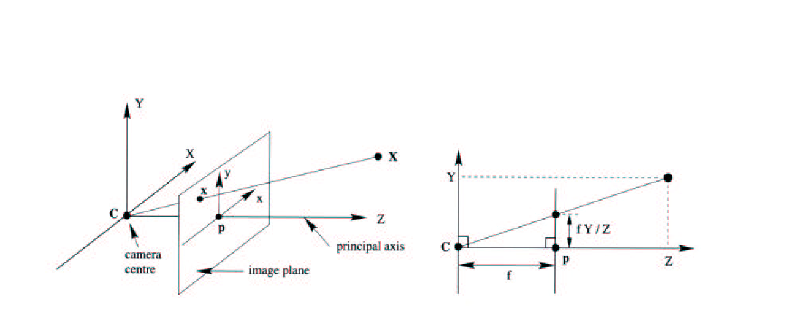
\includegraphics[scale=0.8,keepaspectratio=true]{chap2/pinhole.png}
\caption{The pinhole camera model}
\label{fig:pinhole}
\end{figure}

Represented as homogeneous vectors, the mapping from Euclidean 3-space R3 to Euclidean 2-space R2 can be expressed in matrix multiplication as
$$
\begin{pmatrix}
  fx \\
  fy \\
  z  \\
\end{pmatrix} =
\begin{bmatrix}
   f & 0 & 0 & 0 \\
   0 & f & 0 & 0 \\
   0 & 0 & 1 & 0 \\
\end{bmatrix}
\begin{pmatrix}
  x \\
  y \\
  z \\
  1 \\
\end{pmatrix}
$$
The above formulation assumes that the origin of coordinates in the image plane coincides with the principal point, to account for this offset, where the coordinate of the principal point occurs at 
$(x_0  , y_0)^T$, the mapping 
$$(x, y, z)^T  \rightarrow  (f x/z + x_0, f y/z + y_0)^T$$
can be rewritten as
$$
\begin{pmatrix}
  fx+zx_0 \\
  fy+zy_0 \\
  z  \\
\end{pmatrix} =
\begin{bmatrix}
   f & 0 & x_0 & 0 \\
   0 & f & y_0 & 0 \\
   0 & 0 & 1 & 0 \\
\end{bmatrix}
\begin{pmatrix}
  x \\
  y \\
  z \\
  1 \\
\end{pmatrix}
$$
If we define a matrix K, known as the intrinsic camera matrix since it describes the internal camera parameters,
$$
K = 
\begin{bmatrix}
   f & 0 & x_0 \\
   1 & f & y_0 \\
   1 & 0 & 1 \\
\end{bmatrix}
$$
Then the mapping from R3 to R2 can be written as
$$p = K[ I|0 ]P$$

Furthermore in general, the camera coordinate system is embedded inside a world coordinate frame and the origin of the camera center, C, does not necessary coincides with the world coordinate origin. We realize the the P that we have been referring so far is expressed with respect to the camera coordinate system, and computations are generally performed with respect to the world coordinate system. The 3D point P relates to the world coordinate system by $P = R(P_w - C)$, where R is the rotation matrix representing the orientation of the camera coordinate frame. In matrix form this would become

$$P = \begin{bmatrix} R & -RC \\ 0 & 1 \end{bmatrix} P_w$$

Combining this with the intrinsic camera matrix, we obtain
				$$ P = K R [I |- C]P_w $$

The term $K R [I |- C]$ is the camera projection matrix. It is however more convenient not to explicitly describe the camera center and represent the transformation between the coordinate system as a rotation followed by a translation, giving rise to the more common form of the projection matrix $P$
$P = K [R|t]$

\begin{figure}[htb]
\centering
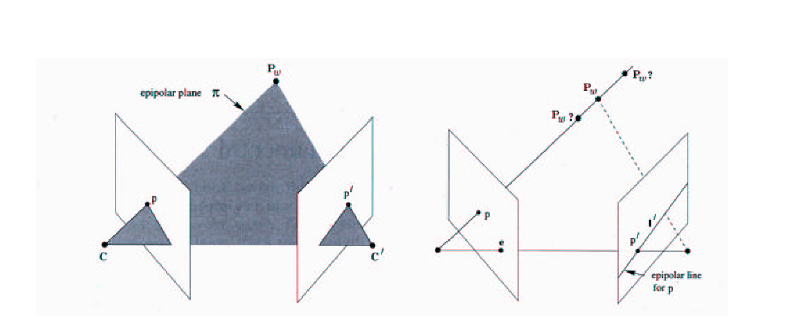
\includegraphics[scale=0.8,keepaspectratio=true]{chap2/epipolar.png}
\caption{Epipolar Geometry}
\label{fig:epipolar}
\end{figure}

Here is a flowchart of mappings from the Voxel Volume to Image Pixels
\begin{figure}[htb]
\centering
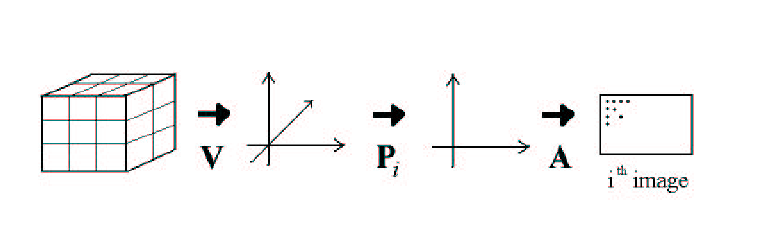
\includegraphics[scale=0.8,keepaspectratio=true]{chap2/flow_chart_voxel.png}
\caption{A flowchart of mappings from the Voxel Volume to Image Pixels}
\label{fig:flow_chart_voxel}
\end{figure}

In our formulation, we will assume a pinhole camera model and that all surfaces are Lambertian (i.e. the radiance observed of a 3D point is independent of viewing direction). The projective coordinate of a 3D point Pw in world space is expressed with homogeneous coordinates as
			$$P_w = \begin{bmatrix} x_w & y_w & z_w \end{bmatrix}^T$$
while the projective image coordinate of a pixel in image i is
$$ p_i = \begin{bmatrix} x_i & y_i & z_i & 1 \end{bmatrix}^ T $$
such that the corresponding pixel coordinate p`i of the projected point pi can be obtained by applying a homogenising function H where 

$$
H
(
\begin{bmatrix}
   x \\
   y \\
   z \\
\end{bmatrix}
)
=
\begin{bmatrix}
   x/z \\
   y/z \\
\end{bmatrix}
$$

Results:
\begin{figure}[htb]
\centering
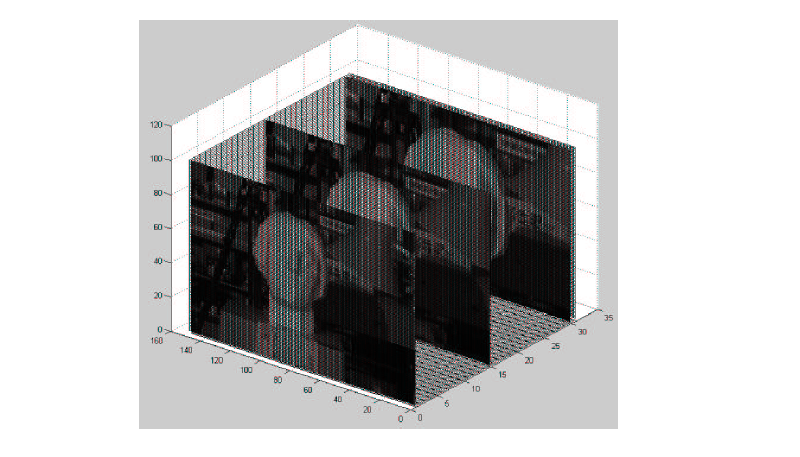
\includegraphics[scale=0.8,keepaspectratio=true]{chap2/projective_volume.png}
\caption{Projective volume projection for one of the image in the 'Head and Lamp' sequence}
\label{fig:projective_volume}
\end{figure}

			

	\item	Metric Volume:

   After the projective volume is determined, a metric volume condensing the feature vectors of each voxel into a meaning measure or matching functional is required. While it is very important for the camera calibration process to determine the correct camera projection matrices so that the projective volume can be correct constructed, it is also very important to select an appropriate metric such that the correct measure can be computed. Accurate projections provide the necessary information for each voxel, so that each voxel can confidently locate the pixels from which it is back-projected to. Given all the information, feature vectors, it is up to the metric volume stage to analyze the obtained information and to decide whether a voxel is part of the 3D object scene. Volumetric scene reconstruction techniques recover depth information by labeling a voxel with either transparent or opaque, or in the case of a ternary decision, as either transparent, opaque or unseen. In the end, the most important task of the reconstruction is this decision. Thus the metric measure has the important task of making this decision through the analysis of the information available. Although our proposed reconstruction technique delays this decision making till the segmentation stage, since segmentation is accomplished through minimization of an energy function, it is still extremely important for the metric volume to derive a meaning measure of cost so that the 3D true scene surface is the global minima.
	
\end{enumerate}

\section{Similar Projects}


\section{What is different with our project?}
